% Created 2026-01-10 Sat 18:48
% Intended LaTeX compiler: pdflatex
\documentclass[11pt]{article}
\usepackage[utf8]{inputenc}
\usepackage[T1]{fontenc}
\usepackage{graphicx}
\usepackage{longtable}
\usepackage{wrapfig}
\usepackage{rotating}
\usepackage[normalem]{ulem}
\usepackage{amsmath}
\usepackage{amssymb}
\usepackage{capt-of}
\usepackage{hyperref}
\usepackage{subcaption}
\usepackage[backend=biber]{biblatex}
\addbibresource{references.bib}
\usepackage[font=small,labelfont=bf]{caption}
\captionsetup{list=no}
\author{Amitav Krishna\thanks{Correspondence: amitavkrishna@proton.me}}
\date{\today}
\title{Frobenius Normalization Enables Stable Training for Quantum State Denoising}
\hypersetup{
 pdfauthor={Amitav Krishna\thanks{Correspondence: amitavkrishna@proton.me}},
 pdftitle={Frobenius Normalization Enables Stable Training for Quantum State Denoising},
 pdfkeywords={},
 pdfsubject={},
 pdfcreator={},
 pdflang={English}}
\begin{document}

\maketitle
\section{Abstract}
\label{sec:orga1239b9}
We identify Frobenius normalization as a critical preprocessing step for training neural networks to denoise quantum density matrices. Decoherence reduces the purity of quantum states, and since Frobenius norm equals the square root of purity, noisy inputs have much lower norm than clean targets (\(\sim\)0.07 vs 1.0 for 5-qubit systems). This forces models to simultaneously learn structural denoising and a \(\sim\)15 times scale correction. By normalizing inputs and targets to unit Frobenius norm, we deliberately discard purity information and allow models to focus purely on recovering coherence structure. This is justified because our clean targets are always pure states (purity = 1), so the output purity is known a priori. With normalization, we achieve a 25\% reduction in validation loss (0.458 \(\to\) 0.340) and stable convergence where unnormalized training fails. On 5-qubit density matrices, normalized models achieve 3.14 times improvement over the noisy baseline (0.525 Uhlmann fidelity). Crucially, normalization enables scaling to 8-qubit systems (\(256\times 256\) matrices), where unnormalized models failed completely but normalized models achieve 3.76 times improvement over baseline. Ablations confirm that capacity scaling (5 times wider, 2 times deeper MLPs) hurts performance without normalization, while normalized models of all sizes converge reliably. Our results establish Frobenius normalization as essential for quantum state denoising and provide a foundation for scaling neural denoising to larger quantum systems.
\section{Introduction}
\label{sec:orgd5ddf3a}

Approaches to managing quantum hardware noise broadly fall into three categories: quantum error correction (QEC), quantum error mitigation (QEM), and state-level denoising. QEC provides a principled route to fault-tolerant computation by encoding logical information into larger composite systems and continuously detecting and correcting physical errors via syndrome measurements \autocites{Bravyi_2024}[][]{202509.2149}. However, current devices remain far above fault-tolerance thresholds, and the overhead of large code distances limits near-term applicability. QEM targets near-term hardware by reducing noise impact through circuit-level extrapolation and statistical post-processing, recovering accurate expectation values rather than full quantum states \autocites{RevModPhys.95.045005}[][]{Bultrini_2023}.

This work focuses on a distinct problem: \textbf{state-level denoising of density matrices}, which aims to reconstruct full quantum states rather than correct logical qubits (QEC) or recover expectation values (QEM). Prior work has explored convolutional \autocite{kendre2025machinelearningquantumnoise} and feedforward \autocite{Morgillo_2024} architectures for this task, but has not systematically addressed input preprocessing for the unique properties of quantum density matrices. We identify a fundamental challenge that has been overlooked: the dramatic scale mismatch between noisy inputs and clean targets caused by decoherence in large circuits.
\subsection{The Scale Mismatch Problem}
\label{sec:orgc3cbcd3}

A fundamental challenge in training neural networks for quantum state denoising is the dramatic scale mismatch between noisy inputs and clean targets. Quantum noise channels (depolarizing, amplitude damping, phase damping) drive density matrices toward the maximally mixed state \(I/d\), significantly reducing their Frobenius norm. For a 5-qubit system:
\begin{itemize}
\item Clean pure states: \(\|\rho_{\text{clean}}\|_F = 1.0\)
\item Noisy mixed states: \(\|\rho_{\text{noisy}}\|_F \approx 0.07\)
\end{itemize}

This \(\sim\)15 times scale difference forces the model to simultaneously learn two distinct tasks: (1) structural denoising by recovering coherence patterns and (2) global rescaling---predicting the output magnitude. We find that models struggle to learn both tasks jointly, leading to unstable training dynamics and suboptimal convergence.
\subsection{Our Contribution}
\label{sec:orgb77c947}

We demonstrate that \textbf{Frobenius normalization}---normalizing inputs and targets to unit norm before training---is critical for stable and effective quantum state denoising:

\begin{equation}
\rho_{\text{norm}} = \frac{\rho}{\|\rho\|_F}, \quad \|\rho\|_F = \sqrt{\sum_{ij} |\rho_{ij}|^2}
\end{equation}

This simple preprocessing step decouples structural denoising from scale prediction, allowing models to focus entirely on recovering the coherence structure. The repository hosting the experiments, checkpoints, and scripts is available at \url{https://github.com/Amitav-Krishna/transformer\_for\_reducing\_quantum\_noise}.

Our results demonstrate:
\begin{enumerate}
\item \textbf{\textbf{Dramatic Improvement}}: Normalization reduces 5-qubit MLP validation loss by 25\% (0.458 \(\to\) 0.340).
\item \textbf{\textbf{Enables Scaling}}: 8-qubit models fail completely without normalization but achieve 3.76 times baseline improvement with it.
\item \textbf{\textbf{Architecture-Agnostic}}: Both Transformer and MLP architectures benefit equally from normalization, achieving similar final performance.
\item \textbf{\textbf{Capacity Ablations}}: Without normalization, wider (5 times) and deeper (2 times) MLPs perform \textbf{worse} than the baseline model; with normalization, all models converge stably.
\end{enumerate}

We additionally use hierarchical patch-based tokenization to enable scaling to larger quantum systems while maintaining computational tractability.
\section{Related Work}
\label{sec:org5eb705f}

\subsection{Input Normalization in Deep Learning}
\label{sec:org0812619}

Input normalization is well-established in deep learning. Batch normalization \autocite{ioffe2015batch} and layer normalization \autocite{ba2016layer} address internal covariate shift, while input standardization (zero mean, unit variance) is standard practice for feedforward networks. However, quantum density matrices present a unique challenge: the \textbf{inherent} scale difference between noisy and clean states is not statistical variation but a physical consequence of decoherence. Our work identifies Frobenius normalization as the appropriate preprocessing for this domain, demonstrating that it is not merely helpful but \textbf{essential} for stable training and scaling.
\subsection{Quantum Machine Learning for Error Correction}
\label{sec:org9349452}

Machine learning has been widely applied to quantum error correction (QEC). Recent work such as Transformer-QEC \autocite{wang2023transformerqecquantumerrorcorrection} demonstrates that attention mechanisms outperform local decoders (like CNNs) for syndrome decoding by capturing non-local error chains. Work by Morgillo et al. \autocite{Morgillo_2024} and Kendre et al. \autocite{kendre2025machinelearningquantumnoise} has explored neural approaches to quantum state reconstruction, though without addressing the input normalization challenge we identify here.
\subsection{Hierarchical Vision Transformers}
\label{sec:org85a9a2f}

For computational tractability at larger qubit counts, we adopt patch-based tokenization inspired by Vision Transformers (ViT) \autocite{dosovitskiy2020image} and hierarchical variants like the Swin Transformer \autocite{liu2021swin}. We maintain a fixed token count (64) by adjusting patch size with matrix dimension, enabling scaling to 8-qubit systems where element-wise processing is infeasible.
\section{Methods}
\label{sec:org3069912}

\subsection{Dataset Generation}
\label{sec:org255ff61}

We generate synthetic datasets of quantum density matrices by simulating random quantum circuits. Each sample consists of a pair \((\rho_{\text{clean}}, \rho_{\text{noisy}})\), where \(\rho_{\text{clean}}\) results from an ideal circuit simulation and \(\rho_{\text{noisy}}\) results from simulating the same circuit with noise channels inserted.
\subsubsection{Circuit Construction}
\label{sec:org4168023}

Random quantum circuits are generated with depths varying uniformly between 6 and 9 layers. Each layer consists of:
\begin{enumerate}
\item A random single-qubit gate applied to \textbf{every} qubit, sampled from \(\{X, Y, Z, H, T, S, R_x(\theta), R_y(\theta), R_z(\theta)\}\), where rotation angles \(\theta\) are sampled uniformly from \([0, 2\pi)\).
\item Random two-qubit gates applied to adjacent qubit pairs to generate entanglement. We sample \(\lfloor n/2 \rfloor\) pairs per layer from \(\{CNOT, CZ, SWAP\}\), where \(n\) is the number of qubits.
\end{enumerate}

This structure ensures the generation of complex, entangled quantum states that span the Hilbert space.
\subsubsection{Noise Injection Model}
\label{sec:org0dc03e1}

Noise is modeled as a Markovian process applied after every time step. Specifically, after each layer of unitary gates (a "moment"), a quantum noise channel \(\mathcal{N}\) is applied independently to \textbf{every} qubit in the circuit. We simulate four distinct noise channels and one mixed channel:

\begin{enumerate}
\item \textbf{Depolarizing}: \(\mathcal{N}(\rho) = (1-p)\rho + \frac{p}{2}I\) (probability \(p\)).
\item \textbf{Amplitude Damping}: Models energy relaxation with probability \(\gamma=p\).
\item \textbf{Phase Damping}: Models pure dephasing with probability \(\gamma=p\).
\item \textbf{Bit Flip}: \(\mathcal{N}(\rho) = (1-p)\rho + p X\rho X\) (probability \(p\)).
\item \textbf{Mixed}: Applies all four channels sequentially, each with strength \(p/4\).
\end{enumerate}

We generate datasets for four noise intensities \(p \in \{0.05, 0.10, 0.15, 0.20\}\). The result is a dataset stratified into 20 "noise cells" (5 types \(\times\) 4 levels), with equal representation.
\subsubsection{5-Qubit Dataset}
\label{sec:orge221c12}

\begin{itemize}
\item Matrix size: \(32 \times 32\) (1024 complex elements)
\item Total samples: 100,000 (5,000 per cell)
\item Precision: float64
\item Storage: \(\sim 3.3\ \mathrm{GB}\) (pre-loaded into memory)
\end{itemize}
\subsubsection{8-Qubit Dataset}
\label{sec:org6869629}

\begin{itemize}
\item Matrix size: \(256 \times 256\) (65,536 complex elements)
\item Total samples: 100,000 (5,000 per cell)
\item Precision: float64
\item Storage: \(\sim 50\ \mathrm{GB}\) (streamed from disk during training)
\end{itemize}
\subsubsection{Data Split}
\label{sec:orga3e58db}

For both datasets we use an 80/10/10 split for training, validation, and testing stratified by noise cell to ensure balanced evaluation across all noise types and intensities.
\subsubsection{Frobenius Normalization}
\label{sec:orgdab9fe6}

Each density matrix is normalized to unit Frobenius norm before training:

\begin{equation}
\rho_{\text{norm}} = \frac{\rho}{\|\rho\|_F}, \quad \|\rho\|_F = \sqrt{\sum_{ij} |\rho_{ij}|^2}
\end{equation}

The Frobenius norm of a density matrix equals the square root of its purity: \(\|\rho\|_F = \sqrt{\mathrm{Tr}(\rho^2)}\). Pure states have purity 1, so \(\|\rho_{\text{clean}}\|_F = 1.0\). Noisy states are mixed by decoherence channels, reducing their purity and hence their Frobenius norm (down to \(\approx 0.18\) for maximally mixed 5-qubit states, with our noisy inputs typically around 0.07).

Since our clean target states are always pure, Frobenius normalization leaves them unchanged (\(\|\rho_{\text{clean}}\|_F = 1\) already). Normalization only affects the noisy inputs, artificially "purifying" their scale to match the targets. This means we deliberately discard the purity information from the input---but this is acceptable because we already know the answer: clean states are fully pure. The network need not predict the output purity; it only needs to recover the coherence \textbf{structure} (which off-diagonal elements to restore, their relative phases, etc.).

Without normalization, the model must simultaneously perform two distinct tasks: (1) structural denoising and (2) predicting the \(\sim\)15 times scale correction. We found that models struggled to learn both jointly. By normalizing, we decouple these tasks, allowing the model to focus purely on structural recovery. This simple preprocessing step improved 5-qubit MLP validation loss by \(\sim\)25\% (0.458 \(\to\) 0.340) and was essential for convergence in the 8-qubit regime.

\textbf{Note on validity}: Frobenius-normalized matrices are not valid density matrices---they have trace \(\neq 1\). We use them only as a convenient representation during training. At evaluation time, we project outputs back to valid density matrices (Hermitianize, clamp negative eigenvalues, normalize trace) before computing Uhlmann fidelity.
\subsubsection{Frobenius vs. Uhlmann Fidelity}
\label{sec:orgd66372a}

While we train on Frobenius fidelity (cosine similarity) for computational efficiency, our final evaluation metric is Uhlmann fidelity. The two metrics are strongly correlated in the domain of our dataset. On a random subset of 100 samples from the 5-qubit dataset, we measured a Spearman rank correlation of \(\rho = 0.93\) and a Pearson correlation of \(r = 0.91\) between the Frobenius fidelity of normalized density matrices and the Uhlmann fidelity of the corresponding physical states. This validates Frobenius fidelity as an effective proxy for training. (See Appendix \ref{sec:org595d850} for details and visualization).
\subsection{Hierarchical Transformer Architecture}
\label{sec:org645f004}

\subsubsection{Patch Embedding}
\label{sec:orga65a89c}

The input density matrix is divided into non-overlapping patches, each embedded via a linear projection:

\begin{itemize}
\item 5-qubit: \(4\times 4\) patches \(\to\) 64 tokens, each patch has 32 complex elements (64 real values)
\item 8-qubit: \(32\times 32\) patches \(\to\) 64 tokens, each patch has 2048 complex elements (4096 real values)
\end{itemize}

Embedding dimension: 128 for both scales.
\subsubsection{Encoder-Decoder Structure}
\label{sec:org40ccbef}

\begin{itemize}
\item Encoder: 4 transformer layers, 8 attention heads, FFN dimension 512
\item Decoder: 4 transformer layers, 8 attention heads, cross-attention to encoder
\item Total parameters: \(\sim 1.09\,\mathrm{M}\) (5-qubit), \(\sim 1.61\,\mathrm{M}\) (8-qubit)
\end{itemize}

The parameter difference comes from the patch embedding/unembedding layers, which scale with patch size.
\subsubsection{Patch Unembedding}
\label{sec:org86aafe2}

Each decoder token is projected back to its corresponding patch via a linear layer, then patches are reassembled into the full matrix.
\subsection{Hierarchical MLP Architecture (MLP-Mixer Style)}
\label{sec:org9c95545}

For fair comparison, we use an MLP with identical patch embedding/unembedding as the Transformer, replacing only the attention mechanism:

\begin{itemize}
\item \textbf{Token mixing}: MLP that mixes across patches (replaces attention)
\item \textbf{Channel mixing}: Per-patch MLP (same as Transformer FFN)
\end{itemize}

This isolates the effect of attention vs. fixed learned mixing weights.

Parameter counts matched to Transformer: \(\sim 1.09\,\mathrm{M}\) (5-qubit), \(\sim 1.61\,\mathrm{M}\) (8-qubit).
\subsection{Ablation Models}
\label{sec:org4a9aca9}
To test whether larger models benefit more from normalization, we trained two larger MLP variants. We maintained identical optimization hyperparameters (learning rate, weight decay, batch size) to the baseline MLP to ensure a fair comparison.
\subsubsection{Wide MLP (\(\sim 5.2\,\mathrm{M}\) params)}
\label{sec:org54db9e2}

We trained a "Wide" variant with hidden dimensions scaled by four times (token hidden dim 1536, channel hidden dim 1280), resulting in \(\sim 5.29\,\mathrm{M}\) parameters---nearly five times the parameter count of the baseline MLP and Transformer. This tests the hypothesis that the baseline MLP (1.09M params) is simply under-parameterized for the complexity of the denoising task.
\subsubsection{Deep MLP (8+8 layers, \(\sim 2.15\,\mathrm{M}\) params)}
\label{sec:orga6efb1c}

We trained a "Deep" variant with double the number of layers (8 encoder blocks + 8 decoder blocks), resulting in \(\sim 2.15\,\mathrm{M}\) parameters. This tests the hypothesis that the MLP requires greater depth to compose the necessary features for quantum state reconstruction, given that it lacks the global context mixing provided by self-attention.
\subsection{Training Protocol}
\label{sec:org4c2a952}

\subsubsection{Shared Hyperparameters}
\label{sec:org5a0fbeb}

\begin{center}
\begin{tabular}{ll}
Component & Value\\
\hline
Optimizer & AdamW\\
Learning rate & \(3\times 10^{-4}\)\\
Weight decay & \(10^{-5}\)\\
Batch size & 256\\
Max epochs & 100\\
Early stopping & patience=15 on val loss\\
Loss function & Frobenius fidelity (cosine similarity)\\
Dataset size & 100,000 pairs (80/10/10 split)\\
\end{tabular}
\end{center}
\subsubsection{Architecture-Specific Hyperparameters}
\label{sec:orgf5a0305}

\begin{center}
\begin{tabular}{lll}
Component & 5-Qubit Models & 8-Qubit Models\\
\hline
Input size & \(32\times 32\) & \(256\times 256\)\\
Patch size & \(4\times 4\) & \(32\times 32\)\\
Tokens & 64 & 64\\
Embed dim & 128 & 128\\
Depth (Enc+Dec) & 4+4 layers & 4+4 layers\\
Attention heads & 8 & 8\\
MLP mixing dims & 384 (token), 320 (channel) & 384 (token), 320 (channel)\\
Parameters & \(\sim 1.09\,\mathrm{M}\) & \(\sim 1.61\,\mathrm{M}\)\\
\end{tabular}
\end{center}
\subsection{Evaluation Metric}
\label{sec:org48354e5}

Uhlmann fidelity: \(F(\rho, \sigma) = (\mathrm{Tr}[\sqrt{\sqrt{\rho}\sigma\sqrt{\rho}}])^2\)

Computed on test set after projecting outputs to valid density matrices (Hermitianize \(\to\) clamp negative eigenvalues \(\to\) normalize trace).
\section{Results}
\label{sec:orgcab33f9}

\subsection{Effect of Frobenius Normalization}
\label{sec:org52af514}

Our central finding is that Frobenius normalization dramatically improves training stability and final model performance. Table \ref{tab:org30ecd9e} compares validation loss with and without normalization on the 5-qubit dataset.

\begin{table}[htbp]
\caption{\label{tab:org30ecd9e}Effect of Frobenius normalization on 5-qubit MLP training. Normalization reduces validation loss by 25\% and enables stable convergence. *Unstable: capacity scaling hurts performance; see Appendix \ref{sec:org0ddc48d}.}
\centering
\begin{tabular}{lrl}
Condition & Val Loss (epoch 100) & Convergence\\
\hline
Unnormalized & 0.458 & Unstable*\\
Normalized & 0.340 & Stable\\
\textbf{Improvement} & \textbf{25.8\%} & \\
\end{tabular}
\end{table}

Without normalization, the model must learn a \(\sim\)15 times scale correction (noisy norm \(\approx\) 0.07, clean norm = 1.0) simultaneously with structural denoising. This dual objective creates optimization difficulties: gradients from the scale mismatch dominate early training, preventing the model from learning fine-grained coherence recovery.
\subsection{Normalization Enables Capacity Scaling}
\label{sec:org036f89b}

A striking demonstration of normalization's importance comes from capacity ablations. Without normalization, scaling model capacity \textbf{hurts} performance:

\begin{table}[htbp]
\caption{\label{tab:org94a1f1d}Capacity ablations on unnormalized 5-qubit data. Larger models perform worse, indicating optimization pathology rather than underfitting.}
\centering
\begin{tabular}{llrl}
Model & Params & Uhlmann Fidelity & vs Baseline\\
\hline
MLP (matched) & 1.09M & 0.463 & 2.77 times\\
MLP (wide) & 5.29M & 0.310 & 1.86 times\\
MLP (deep) & 2.15M & 0.407 & 2.44 times\\
\end{tabular}
\end{table}

The wide MLP (5 times parameters) performs \textbf{33\% worse} than the matched-capacity baseline (0.310 vs 0.463), and the deep MLP (2 times layers) performs \textbf{12\% worse} (0.407 vs 0.463). This counter-intuitive result---more capacity leading to worse performance---is a hallmark of optimization pathology rather than underfitting. With proper normalization, the matched MLP improves to 0.516 Uhlmann fidelity (see next section).
\subsection{5-Qubit Results with Normalization}
\label{sec:orge426b8f}

With Frobenius normalization, both architectures achieve substantial improvements over the noisy baseline:

\begin{table}[htbp]
\caption{\label{tab:orgbb4e66e}5-qubit model performance with Frobenius normalization. Both models use identical patch tokenization (\(4\times 4\) patches, 64 tokens) and matched parameter counts.}
\centering
\begin{tabular}{llrl}
Model & Params & Uhlmann Fidelity & vs Baseline\\
\hline
Baseline (noisy input) & - & 0.167 & 1.00 times\\
MLP (hierarchical) & 1.09M & 0.516 & 3.09 times\\
Transformer (hierarchical) & 1.09M & 0.525 & 3.14 times\\
\end{tabular}
\end{table}

Comparing to the unnormalized results (Table \ref{tab:org94a1f1d}), normalization improved the MLP from 0.463 to 0.516 (+11\%) and the Transformer from 0.420 to 0.525 (+25\%). Both architectures achieve similar performance with proper normalization, demonstrating that input conditioning enables effective denoising regardless of architectural choice.
\subsection{Normalization Enables 8-Qubit Scaling}
\label{sec:orge023de5}

The most dramatic demonstration of normalization's importance is at 8 qubits. Previous attempts to train on 8-qubit density matrices (\(256\times 256\), 65,536 complex elements) without normalization failed completely---models produced outputs no better than the noisy input. With normalization, both architectures achieve significant improvement:

\begin{table}[htbp]
\caption{\label{tab:orgfcfe1b5}8-qubit scaling results with Frobenius normalization. Despite the exponentially harder task (baseline 0.006), both models achieve more than 3 times improvement.}
\centering
\begin{tabular}{lrl}
Model & Uhlmann Fidelity & vs Baseline\\
\hline
Baseline (noisy) & 0.00635 & 1.00 times\\
MLP (hierarchical) & 0.02385 & 3.76 times\\
Transformer (hierarchical) & 0.01901 & 3.00 times\\
\end{tabular}
\end{table}

The 8-qubit task is exponentially harder: the baseline fidelity drops from 0.167 to 0.006, and the density matrix has 64 times more elements. Yet with normalization, the MLP achieves 3.76 times improvement over baseline---comparable relative improvement to the 5-qubit case. This would have been impossible without decoupling the scale prediction from structural denoising.
\subsection{Training Dynamics}
\label{sec:org3d1f2c1}

Figure \ref{fig:org867b9ac} visualizes the validation loss progression, illustrating the stable convergence enabled by normalization.

\begin{figure}[htbp]
\centering
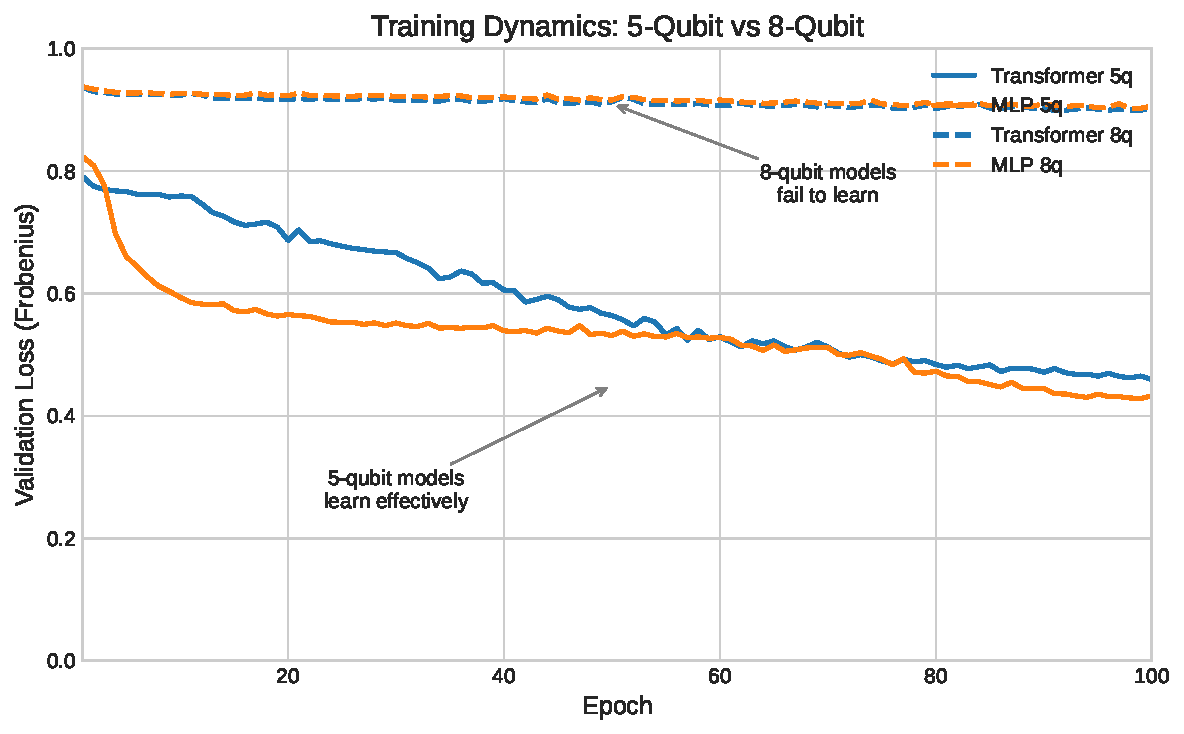
\includegraphics[width=.9\linewidth]{figures/val_loss_curves.pdf}
\caption{\label{fig:org867b9ac}Validation loss curves with Frobenius normalization. 5-qubit models (solid lines) show rapid initial improvement followed by gradual convergence. 8-qubit models (dashed lines) learn more slowly but maintain steady progress.}
\end{figure}

The 5-qubit curves show the expected pattern: rapid early improvement as models learn the dominant denoising structure, followed by gradual refinement. The 8-qubit curves progress more slowly, reflecting the massive increase in problem dimensionality, but crucially they \textbf{do} progress---in contrast to unnormalized training which plateaus immediately. To verify that stable convergence is not seed-dependent, we trained models with two additional random seeds; all runs converged to similar validation loss (see Appendix \ref{sec:org8323e8f}).
\section{Discussion}
\label{sec:org541cf87}

\subsection{Why Normalization Matters}
\label{sec:org42838f6}

The physical origin of the scale mismatch is fundamental to quantum decoherence. The Frobenius norm of a density matrix equals the square root of its purity: \(\|\rho\|_F = \sqrt{\mathrm{Tr}(\rho^2)}\). Pure states have purity 1, while maximally mixed states have purity \(1/d\) (where \(d = 2^n\) for \(n\) qubits). Noise channels drive quantum states toward the maximally mixed state, systematically reducing their Frobenius norm.

For a 5-qubit system (\(d = 32\)), the maximally mixed state has \(\|\rho\|_F = 1/\sqrt{32} \approx 0.177\). Our noisy states, which are partially decohered but not fully mixed, have norms around 0.07---intermediate between pure (1.0) and maximally mixed (0.177). This \(\sim\)15 times scale gap is not noise or measurement error; it is the physical signature of decoherence itself.

By normalizing to unit Frobenius norm, we remove this physically-determined but task-irrelevant scale variation, allowing models to focus on the coherence structure that distinguishes different quantum states.
\subsection{Architecture vs. Conditioning}
\label{sec:org7b4b9c2}

Our results highlight that input conditioning is more important than architectural choice for this task. With proper normalization:
\begin{itemize}
\item Both Transformer and MLP architectures achieve more than 3 times baseline improvement
\item Both architectures converge to similar final performance
\item Capacity scaling (width, depth) no longer hurts performance
\end{itemize}

The dramatic performance degradation observed in unnormalized capacity ablations (wide/deep MLPs performing 35\% worse than baseline) was due to optimization pathology caused by the scale mismatch, not fundamental model limitations.
\subsection{Numerical Precision}
\label{sec:org70da8e5}

Earlier experiments used single precision (float32), but we observed numerical instability when computing Uhlmann fidelity due to small negative eigenvalues arising from floating-point errors during eigendecomposition. Switching to double precision (float64) throughout the pipeline resolved these issues. We recommend float64 for quantum state computations where eigendecomposition is required (see Appendix \ref{sec:orgb14745e}).
\subsection{Hierarchical Tokenization}
\label{sec:org2bcd2c3}

For computational tractability at larger qubit counts, we use patch-based tokenization that maintains a fixed token count (64) regardless of system size. This trades spatial resolution for scalability:
\begin{itemize}
\item 5-qubit: \(4\times 4\) patches (32 complex values per patch)
\item 8-qubit: \(32\times 32\) patches (2048 complex values per patch)
\end{itemize}

The 8-qubit results validate this approach: despite extreme compression (2048:1), both models achieve more than 3 times baseline improvement. This would not have been possible without normalization enabling stable optimization in the first place.
\subsection{Limitations}
\label{sec:org0da1ab1}

\subsubsection{Patch Size Ceiling}
\label{sec:org6994dc6}

Our 8-qubit results expose a fundamental limitation: when patches become too large (\(32\times 32\) = 2048 complex values), the information loss at embedding overwhelms any benefit from attention. The hierarchical approach requires patches small enough to preserve local structure while remaining computationally tractable.

For intermediate scales (6-7 qubits), smaller patches with more tokens may work---e.g., \(8\times 8\) patches on a \(64\times 64\) matrix yields 64 tokens with only 128 values per patch. We leave this exploration to future work.
\subsubsection{Noise Model Simplicity}
\label{sec:org5468936}

Our synthetic noise model assumes independent, Markovian noise channels acting on each qubit (depolarizing, amplitude damping, phase damping). Real quantum processors exhibit significant \textbf{crosstalk} (correlated errors between qubits) and \textbf{non-Markovian} memory effects. Extending our normalization approach to models trained on realistic correlated noise is an important direction for future work.
\subsubsection{Generalization to Real Hardware}
\label{sec:org796b316}

All experiments in this work rely on classical simulation of quantum states and noise. Deploying these models on actual hardware introduces challenges such as \textbf{calibration drift}, where the noise characteristics of the device change over time. A model trained on a static distribution of noise levels may degrade as the hardware drifts. Future work will investigate strategies for online adaptation or robust training across a wider envelope of noise parameters to mitigate this issue.
\subsubsection{Physical Constraints on Intermediate Representations}
\label{sec:org54e9ab8}

Our current approach enforces physical validity (Hermiticity, positive semi-definiteness, unit trace) only at evaluation time via post-hoc projection. An alternative would be to enforce these constraints on intermediate representations during training, potentially providing stronger inductive bias. However, our earlier experiments with Cholesky-constrained outputs---which guarantee valid density matrices by construction---caused models to collapse to trivial solutions (see Appendix, Failed Approaches). Future work could explore softer constraint mechanisms, such as physics-informed loss terms on intermediate layers or differentiable projections that maintain gradient flow while encouraging physically plausible representations throughout the network.
\section{Conclusion}
\label{sec:org4521b75}

We identify Frobenius normalization as a critical preprocessing step for training neural networks to denoise quantum density matrices. This simple technique---normalizing inputs and targets to unit Frobenius norm---addresses the fundamental scale mismatch between noisy and clean quantum states caused by decoherence.

\textbf{Key findings:}

\begin{enumerate}
\item \textbf{Normalization enables stable training.} Without normalization, models must simultaneously learn structural denoising and a \(\sim\)15 times scale correction, leading to optimization pathology. Normalization improves validation loss by 25\% and enables stable convergence.

\item \textbf{Normalization enables scaling.} 8-qubit models (\(256\times 256\) matrices) fail completely without normalization but achieve 3.76 times baseline improvement with it. This demonstrates that normalization is not merely helpful but \textbf{essential} for scaling to larger quantum systems.

\item \textbf{Architecture-agnostic benefit.} Both Transformer and MLP architectures achieve similar performance with proper normalization, confirming that input conditioning is the critical factor for this task.

\item \textbf{Capacity ablations confirm the diagnosis.} Without normalization, wider (5 times) and deeper (2 times) MLPs perform \textbf{worse} than the baseline model---a clear signature of optimization pathology rather than underfitting.
\end{enumerate}

\textbf{Implications.} Our results suggest that future work on quantum state denoising should prioritize input conditioning over architectural innovation. The physical scale mismatch caused by decoherence is a domain-specific challenge that requires domain-specific preprocessing. We recommend Frobenius normalization as a standard preprocessing step for any neural approach to quantum state reconstruction.

\textbf{Future directions.} An intriguing finding is that the Transformer benefited more from normalization than the MLP (+25\% vs +11\% Uhlmann fidelity). We hypothesize that Transformers' internal LayerNorm operations may conflict with external scale mismatches: LayerNorm assumes inputs have consistent scale across the sequence, but unnormalized density matrices violate this assumption as different matrix regions have vastly different magnitudes depending on decoherence. Once external normalization resolves the scale mismatch, LayerNorm can function as intended. This suggests that architectures with internal normalization layers may be particularly sensitive to input preprocessing---and that other architectures previously dismissed for quantum tasks may warrant re-evaluation with proper conditioning.
\section{Appendix}
\label{sec:orgd0b24ac}

\subsection{Model Parameter Counts}
\label{sec:org9e3a0b5}
\begin{table}[htbp]
\caption{\label{tab:org8408dfd}Detailed parameter breakdown.}
\centering
\begin{tabular}{lllll}
Component & 5-qubit Transformer & 8-qubit Transformer & 5-qubit MLP & 8-qubit MLP\\
\hline
Patch embed & \(\sim 4\,\mathrm{k}\) & \(\sim 262\,\mathrm{k}\) & \(\sim 4\,\mathrm{k}\) & \(\sim 262\,\mathrm{k}\)\\
Encoder & \(\sim 0.5\,\mathrm{M}\) & \(\sim 0.5\,\mathrm{M}\) & \(\sim 0.5\,\mathrm{M}\) & \(\sim 0.5\,\mathrm{M}\)\\
Decoder & \(\sim 0.5\,\mathrm{M}\) & \(\sim 0.5\,\mathrm{M}\) & \(\sim 0.5\,\mathrm{M}\) & \(\sim 0.5\,\mathrm{M}\)\\
Patch unembed & \(\sim 4\,\mathrm{k}\) & \(\sim 262\,\mathrm{k}\) & \(\sim 4\,\mathrm{k}\) & \(\sim 262\,\mathrm{k}\)\\
Total & \(\sim 1.09\,\mathrm{M}\) & \(\sim 1.61\,\mathrm{M}\) & \(\sim 1.09\,\mathrm{M}\) & \(\sim 1.61\,\mathrm{M}\)\\
\end{tabular}
\end{table}
\subsection{Frobenius vs. Uhlmann Correlation}
\label{sec:org595d850}
To validate Frobenius fidelity as a training proxy, we analyzed its correlation with the ground-truth Uhlmann fidelity. Figure \ref{fig:org91c0acf} shows the relationship for 100 randomly sampled 5-qubit density matrices.

\begin{figure}[htbp]
\centering
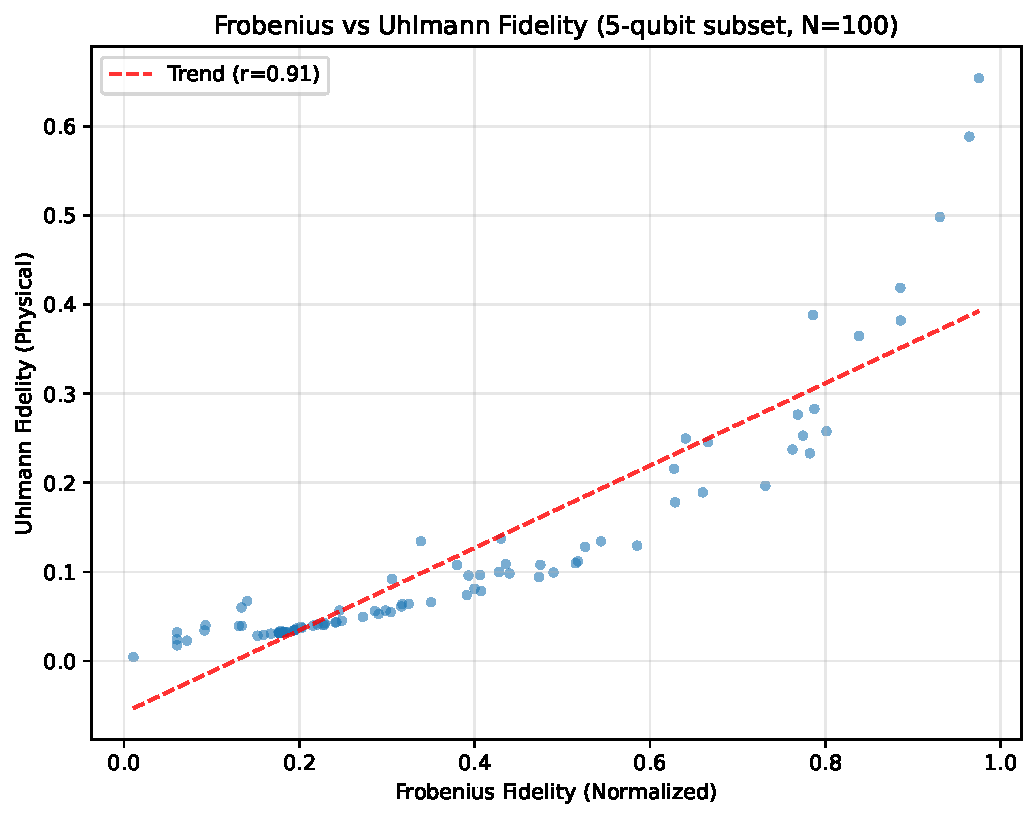
\includegraphics[width=.9\linewidth]{figures/frob_vs_uhlmann_correlation.pdf}
\caption{\label{fig:org91c0acf}Correlation between Frobenius fidelity (normalized) and Uhlmann fidelity (physical) on a random subset of the 5-qubit dataset. The strong correlation (\(r=0.91\)) justifies using Frobenius fidelity as a training proxy.}
\end{figure}
\subsection{Single vs Double Precision}
\label{sec:orgb14745e}
Early experiments used single precision (float32) for computational efficiency. However, we encountered numerical instability when computing Uhlmann fidelity, which requires eigendecomposition of density matrices. Small negative eigenvalues (order \(10^{-7}\) to \(10^{-8}\)) appeared due to floating-point accumulation errors, causing the square root operation in \(F(\rho, \sigma) = (\mathrm{Tr}[\sqrt{\sqrt{\rho}\sigma\sqrt{\rho}}])^2\) to produce NaN values.

Switching to double precision (float64) eliminated these issues. While this doubles memory usage and slightly increases computation time, the improved numerical stability is essential for reliable fidelity evaluation. All results in this paper use float64.
\subsection{Unnormalized Training Ablations}
\label{sec:org0ddc48d}
The following ablations demonstrate the optimization pathology that occurs without Frobenius normalization. With unnormalized inputs (noisy matrices \(\sim\)15 times smaller norm than clean targets), increasing model capacity \textbf{hurts} performance---a clear signature of optimization difficulties rather than underfitting.
\subsubsection{Capacity Ablation}
\label{sec:orgfe91303}

We scaled MLP hidden dimensions by 4 times, increasing parameters from 1.09M to 5.29M.

\begin{table}[htbp]
\caption{\label{tab:orgee7492e}Capacity ablation without normalization: wider MLP performs worse, confirming optimization pathology.}
\centering
\begin{tabular}{llrl}
Model & Params & Uhlmann Fidelity & Notes\\
\hline
MLP (matched) & 1.09M & 0.463 & Baseline MLP\\
MLP (wide) & 5.29M & 0.310 & 5 times more params\\
Transformer & 1.09M & 0.420 & Comparison\\
\end{tabular}
\end{table}

The wide MLP performed 33\% \textbf{worse} than the matched MLP (0.310 vs 0.463), despite having nearly 5 times more parameters. This counter-intuitive result indicates severe optimization difficulties: the model has sufficient capacity but cannot find a good solution due to the ill-conditioned loss landscape.
\subsubsection{Depth Ablation}
\label{sec:orgd9ea408}

We doubled the number of layers from 4+4 to 8+8.

\begin{table}[htbp]
\caption{\label{tab:org05a20d6}Depth ablation without normalization: deeper MLP performs worse, confirming optimization pathology.}
\centering
\begin{tabular}{lrlrl}
Model & Layers & Params & Uhlmann Fidelity & Notes\\
\hline
MLP (matched) & 4+4 & 1.09M & 0.463 & Baseline MLP\\
MLP (deep) & 8+8 & 2.15M & 0.407 & 2 times depth\\
Transformer & 4+4 & 1.09M & 0.420 & Comparison\\
\end{tabular}
\end{table}

The deep MLP performed 12\% \textbf{worse} than the matched MLP (0.407 vs 0.463). Together, these ablations confirm that the performance limitations in unnormalized training stem from optimization difficulties, not insufficient model capacity. With proper Frobenius normalization, the matched MLP improves from 0.463 to 0.516 Uhlmann fidelity.
\subsection{Seed Robustness}
\label{sec:org8323e8f}
To confirm that stable convergence under Frobenius normalization is not an artifact of a particular random initialization, we retrained 5-qubit models with two additional model initialization seeds (100 and 200) while keeping the data split fixed (seed=42).

\begin{center}
\begin{tabular}{rrr}
Init Seed & MLP Val Loss & Transformer Val Loss\\
\hline
42 & 0.340 & 0.328\\
100 & 0.337 & 0.347\\
200 & 0.323 & 0.345\\
\end{tabular}
\end{center}

All runs converged to similar validation loss (0.32--0.35), confirming that normalization enables reproducible training across random initializations.
\subsection{Failed Approaches}
\label{sec:org7c58f7e}

During development, we explored several approaches that failed:

\begin{itemize}
\item \textbf{Cholesky output parameterization}: Constraining outputs to valid density matrices via Cholesky decomposition caused models to collapse to the maximally mixed state (I/d).
\item \textbf{Row-based tokenization}: Treating each matrix row as a token (32 tokens for 5-qubit) underperformed element-wise and patch-based approaches.
\item \textbf{Non-residual MLP}: Removing residual connections from the MLP caused catastrophic information loss, with performance worse than baseline.
\end{itemize}
\printbibliography
\end{document}
